\documentclass[a4paper, 12pt, oneside]{scrartcl}

\usepackage[a4paper, total={7in, 10in}]{geometry}
\usepackage[T2A]{fontenc}            % внутренняя кодировка  TeX
\usepackage[utf8]{inputenc}          % кодовая страница документа
\usepackage[english, russian]{babel} % локализация и переносы

\usepackage{indentfirst}   % русский стиль: отступ первого абзаца раздела
\usepackage{misccorr}      % точка в номерах заголовков
\usepackage{cmap}          % русский поиск в pdf
\usepackage{graphicx}      % Работа с графикой \includegraphics{}
\usepackage{psfrag}        % Замена тагов на eps картинкаx
\usepackage{caption2}      % Работа с подписями для фигур, таблиц и пр.
\usepackage{soul}          % Разряженный текст \so{} и подчеркивание \ul{}
\usepackage{soulutf8}      % Поддержка UTF8 в soul
\usepackage{fancyhdr}      % Для работы с колонтитулами
\usepackage{multirow}      % Аналог multicolumn для строк
\usepackage{ltxtable}      % Микс tabularx и longtable
\usepackage{paralist}      % Списки с отступом только в первой строчке
\usepackage[perpage]{footmisc} % Нумерация сносок на каждой странице с 1
\usepackage{amsmath}  % 
\usepackage{amsfonts}
\usepackage{amssymb}
\usepackage{lipsum}
\usepackage{setspace}

\renewcommand{\baselinestretch}{1.5} 

\begin{document}
	\begin{center}
	{\scshape\Large\bfseries Дальневосточный федеральный университет \par}
	{\scshape\Large Школа естественных наук \par}
	{\large Лабораторная работа №1 по дифференциальным уравнениям \par}
	{\large\bfseries Потоцкая Анастасия Б8203а \par}
	\end{center}
	В лабораторной работе использовалась система компьютерной алгебры wxMaxima. 
		\begin{enumerate}

		\item[1.]
		$$yln(y) + xy' = 0$$
		$$\frac{dy}{yln(y)} = -\frac{dx}{x}$$ 
		\textbf{Тип:}
		дифференциальное уравнение 1-го порядка с разделяющимися переменными \\

		\textbf{Общее решение:}
		$$-\ln{(\ln{(y)})} = \ln{(x)} + C$$

		\textbf{Команды вводимые в wxMaxima: }
		\begin{verbatim}
		ode2('diff(y, x) * x + y * log(y) = 0, y, x);
		method;
		plotdf(-y*log(y)/x, [x, 0.1, 100], [y, 0.1, 100]);
		\end{verbatim} 
		\begin{figure}[ht]
		\center{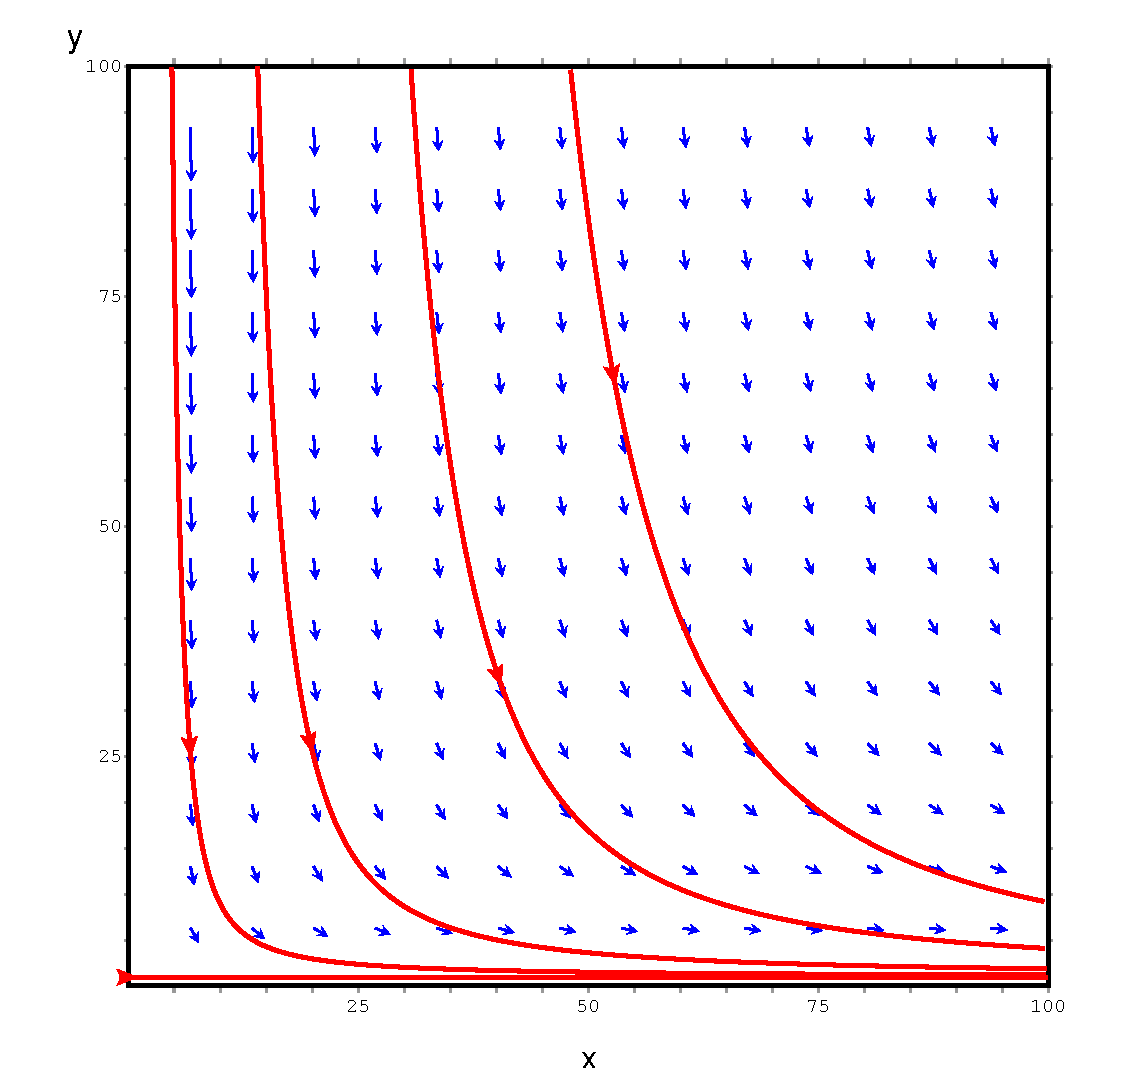
\includegraphics[width=.5\linewidth]{./src/1_2}}
		\captionof{figure}{Векторное поле уравнения $yln(y) + xy' = 0$}
		\end{figure}
		
		\item[2.]
		$$y' = \frac{x + 2y}{2x - y}$$
		$$(2x - y)dy - (x + 2y)dx = 0 $$
		\textbf{Тип: } однородное дифференциальное уравнение 1-го порядка \\
		
		\textbf{Общее решение: }
		$$\frac{4\arctan{(\frac{x}{y})} + \ln{(y^{2} + x^{2}})}{10} = C$$
		
		\textbf{Команды вводимые в wxMaxima }
		\begin{verbatim}
		ode2('diff(y, x) = (x+2*y)/(2*x-y), y, x);
		method;
		plotdf((x+2*y)/(2*x-y), [x, -10, 10], [y, -10, 10]);
		\end{verbatim}
		\begin{figure}[ht]
		\center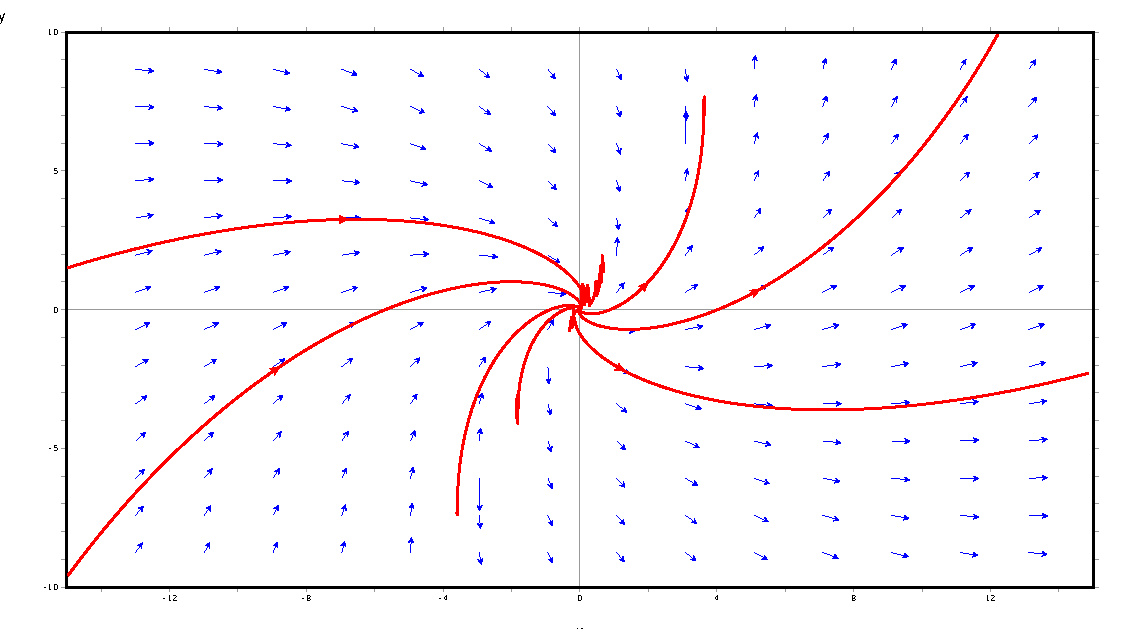
\includegraphics[width=.5\linewidth]{./src/2_2}
		\captionof{figure}{Векторное поле уравнения $y' = \frac{x + 2y}{2x - y}$}
		\end{figure}
		
		\item[3.]
		$$y' = \frac{x + 4y - 5}{6x - y - 5}$$
		$$(6x - y - 5)dy - (x + 4y - 5)dx = 0$$ 
		\textbf{Тип: }
		Обобщенное однородное дифференциальное уравнение 1-го порядка \\
		
		\textbf{Решение: }
		Найти общее решение, которое выражается в элементарных функциях, не удалось \\
		
		\textbf{Команды вводимые в wxMaxima }  
		\begin{verbatim} 
		ode2('diff(y, x) = (x + 4 * y - 5)/(6*x - y - 5) , y, x); 
		method;
		plotdf((x+4*y-5)/(6*x-y- 5), [x, 0, 10], [y, -10, 10]);
		\end{verbatim}
		\begin{figure}[ht]
		\center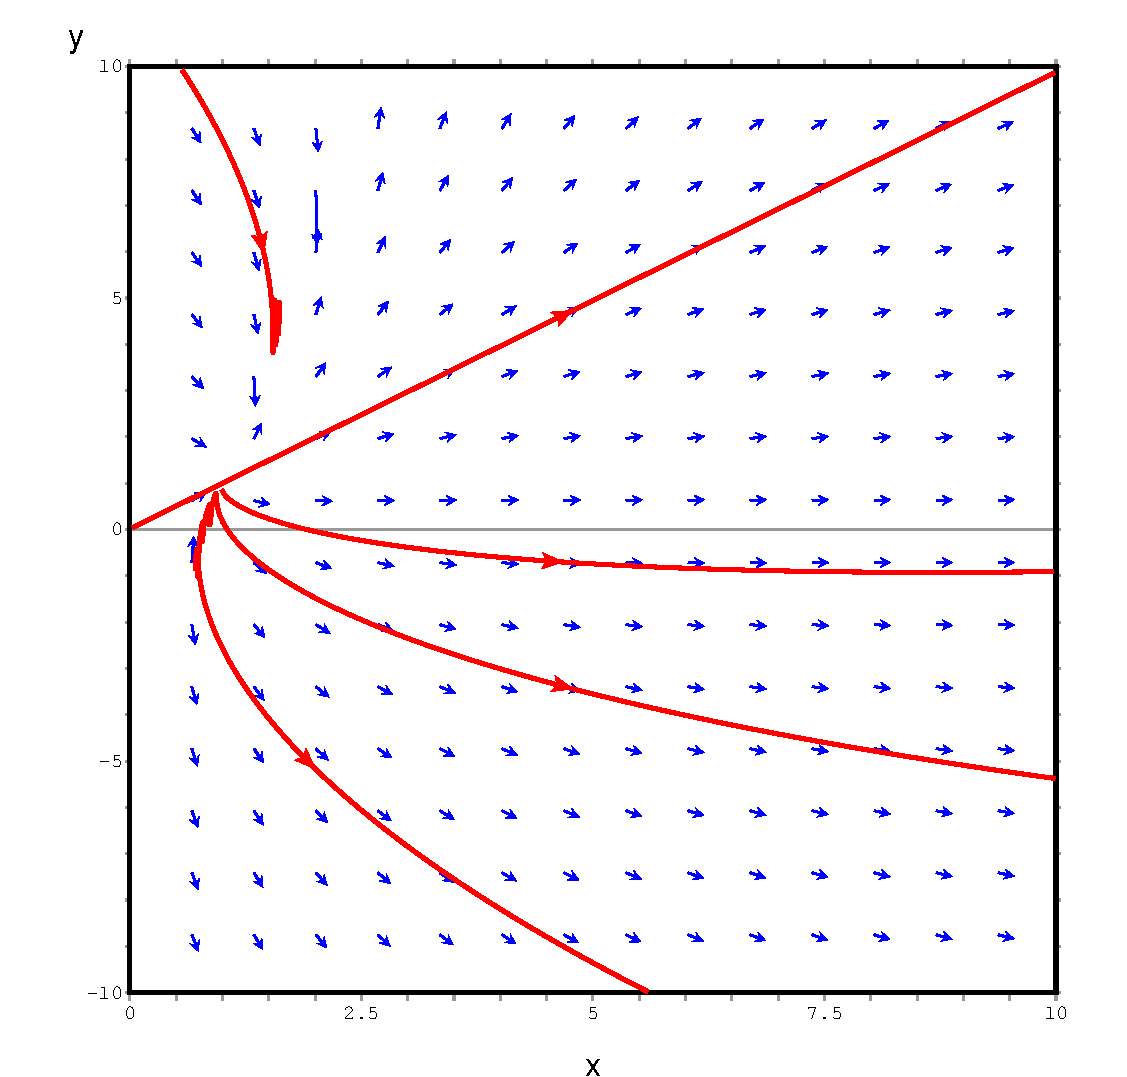
\includegraphics[width=.5\linewidth]{./src/3_}
		\captionof{figure}{Векторное поле уравнения $y' = \frac{x + 4y - 5}{6x - y - 5}$ }
		\end{figure}

		\item[4.]
		$$y' + \frac{2}{x}y = {x^2}; \quad y(1) = -\frac{5}{6}$$
		$$y' + \frac{2}{x}y = {x^2}$$ 
		\textbf{Тип:} линейное дифференциальное уравнение 1-го порядка \\

		\textbf{Общее решение:}
		$$y = -2y\ln{(x)} + \frac{x^{3}}{3} + C $$

		\textbf{Частное решение}
		$$y = -\frac{-773 - 216x^{3} + 1296y(\ln{(x)} - \ln{(-\frac{5}{6})})}{648}$$

		\textbf{Команды вводимые в wxMaxima }
		\begin{verbatim}
		'diff(y, x)+(2 * y)/(x)=x*x;
		ode2(%, y, x);
		method;
		ic1(%, x=-5/6, y=1);
		plotdf(x*x - (2 * y) / (x), [trajectory_at ,-0.833333333, 1]);
		\end{verbatim}
		\begin{figure}[ht]
		\center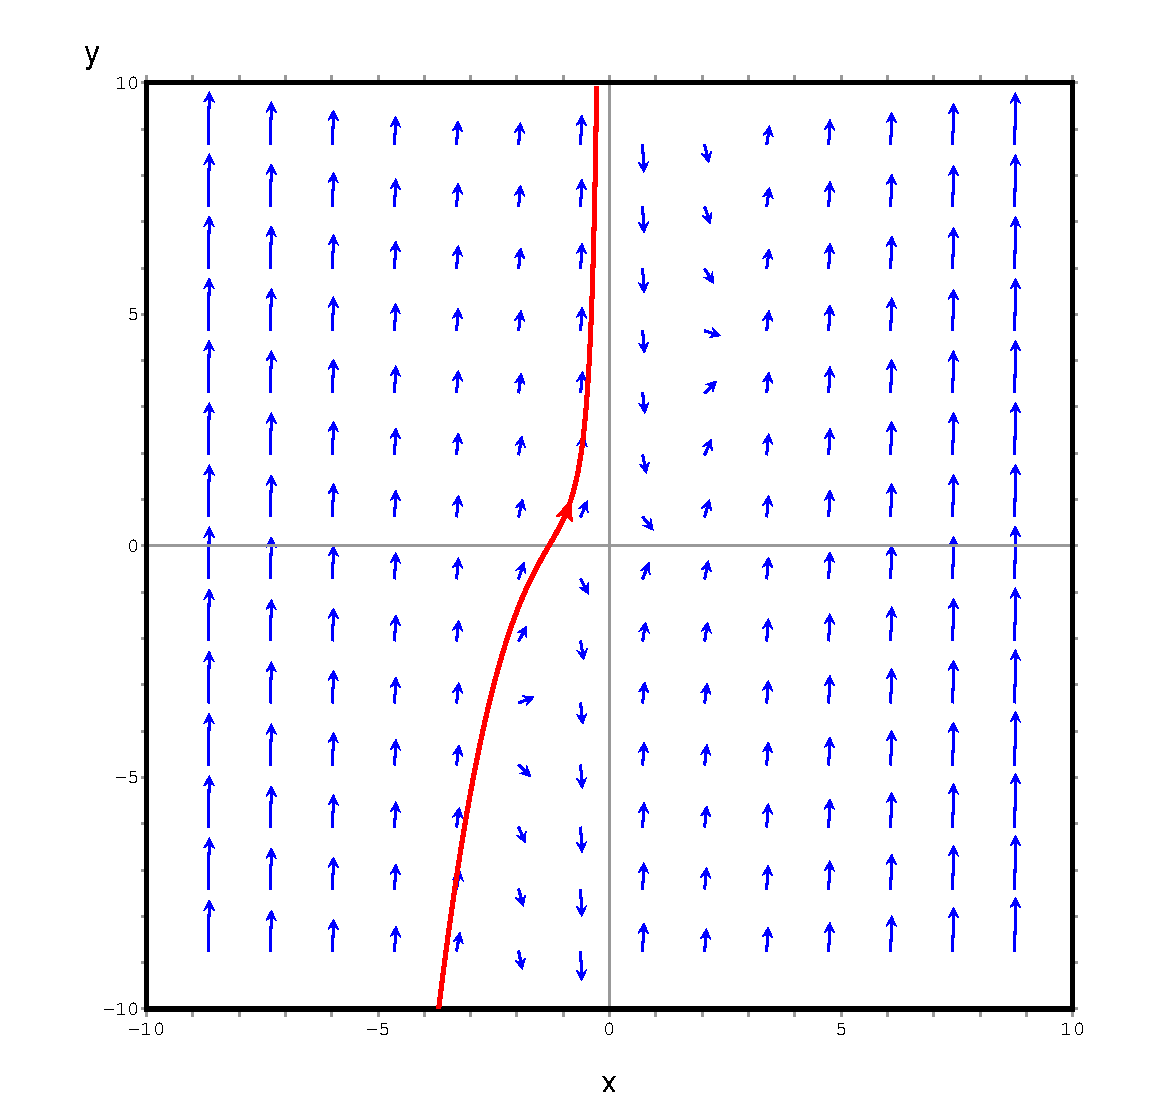
\includegraphics[width=.5\linewidth]{./src/4_}
		\captionof{figure}{Векторное поле уравнения $y' + \frac{2}{x}y = {x^2}$}
		\end{figure}

		\item[5.]
		$$(xy + \sqrt{y})dy + y^{2}dx = 0; \quad y(-\frac{1}{2}) = 4$$
		$$y^{2}x' + xy + \sqrt{y} = 0$$ 
		\textbf{Тип: }
		линейное относительно $x$ дифференциальное уравнение 1-го порядка \\

		\textbf{Общее решение:}
		$$xy + 2\sqrt{y} = C$$ 

		\textbf{Частное решение:}
		$$xy + 2\sqrt{y} = 2$$
		
		\textbf{Команды вводимые в wxMaxima} 
		\begin{verbatim}
		'diff(y, x) = - (y^2) / (x*y + y^(1/2));
		ode2(%, y, x);
		method;
		ic1(%, x=-0.5, y=4);
		plotdf(- (y^2) / (x*y + y^(1/2)), [trajectory_at,-0.50001, 4],[y,2,20],[x,-10,10]);
		\end{verbatim}
		\begin{figure}[ht]
		\center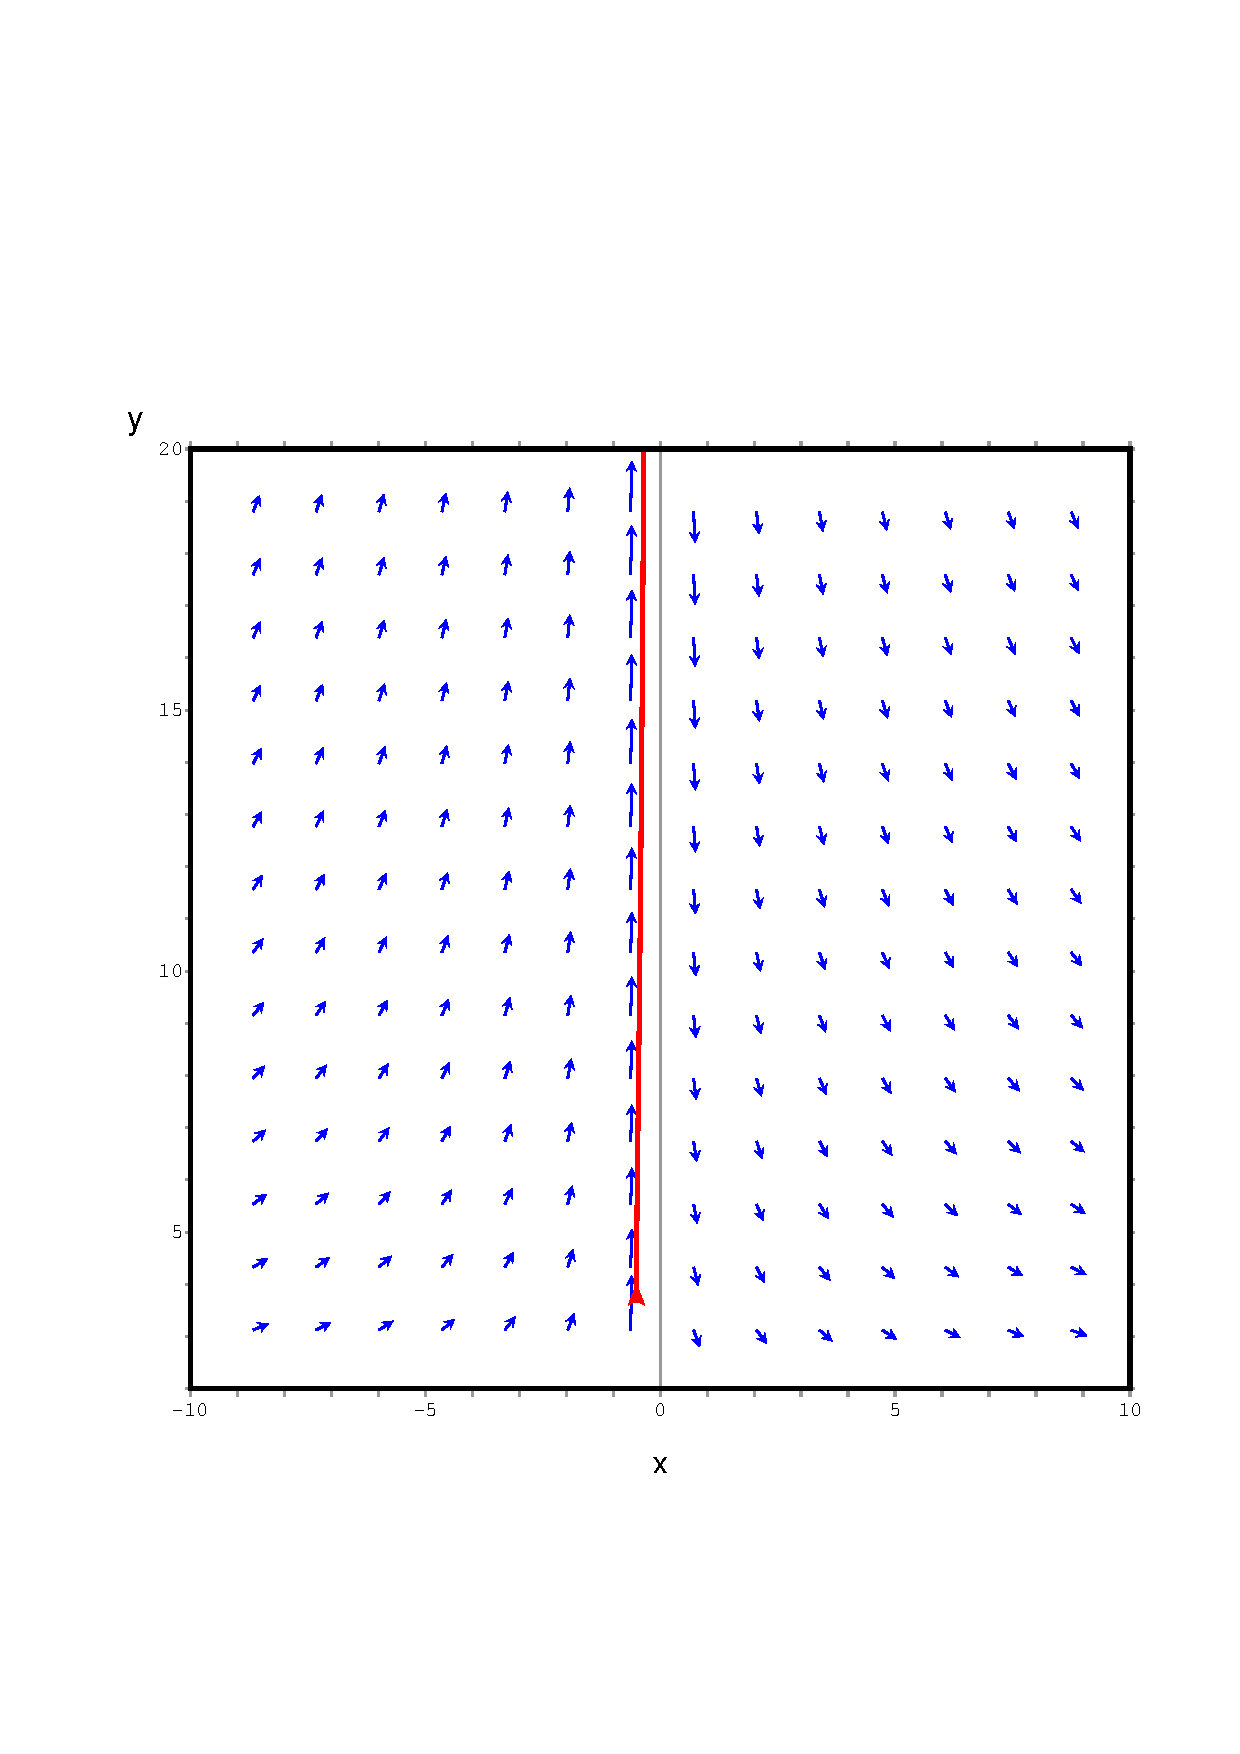
\includegraphics[width=.5\linewidth]{./src/5_2}
		\captionof{figure}{Векторное поле уравнения $(xy + \sqrt{y})dy + y^{2}dx = 0$}
		\end{figure}

		\item[6.]
		$$3(xy' + y) = xy^2; \quad y(1) = 3$$
		$$3y' + 3\frac{y}{x} = y^2$$ 
		\textbf{Тип: }
		уравнение Бернулли \\
		
		\textbf{Общее решение: }
		$$y = \frac{1}{x(C - \frac{\ln{(x)}}{3})}$$

		\textbf{Частное решение: }
		$$y = -\frac{3}{x\ln{x} - x}$$ 
		
		\textbf{Команды вводимые в wxMaxima}
		\begin{verbatim}
		ode2('diff(y(x), x) = y(x)^2 / 3 - y(x) / x, y(x), x);
		method;
		ic1(%, y(x) = 3, x = 1);
		plotdf((y^2)/ 3 - y/x, [trajectory_at, 1, 3], [y, -10,  10], [x, 0, 20]);
		\end{verbatim}

		\begin{figure}[ht]
		\center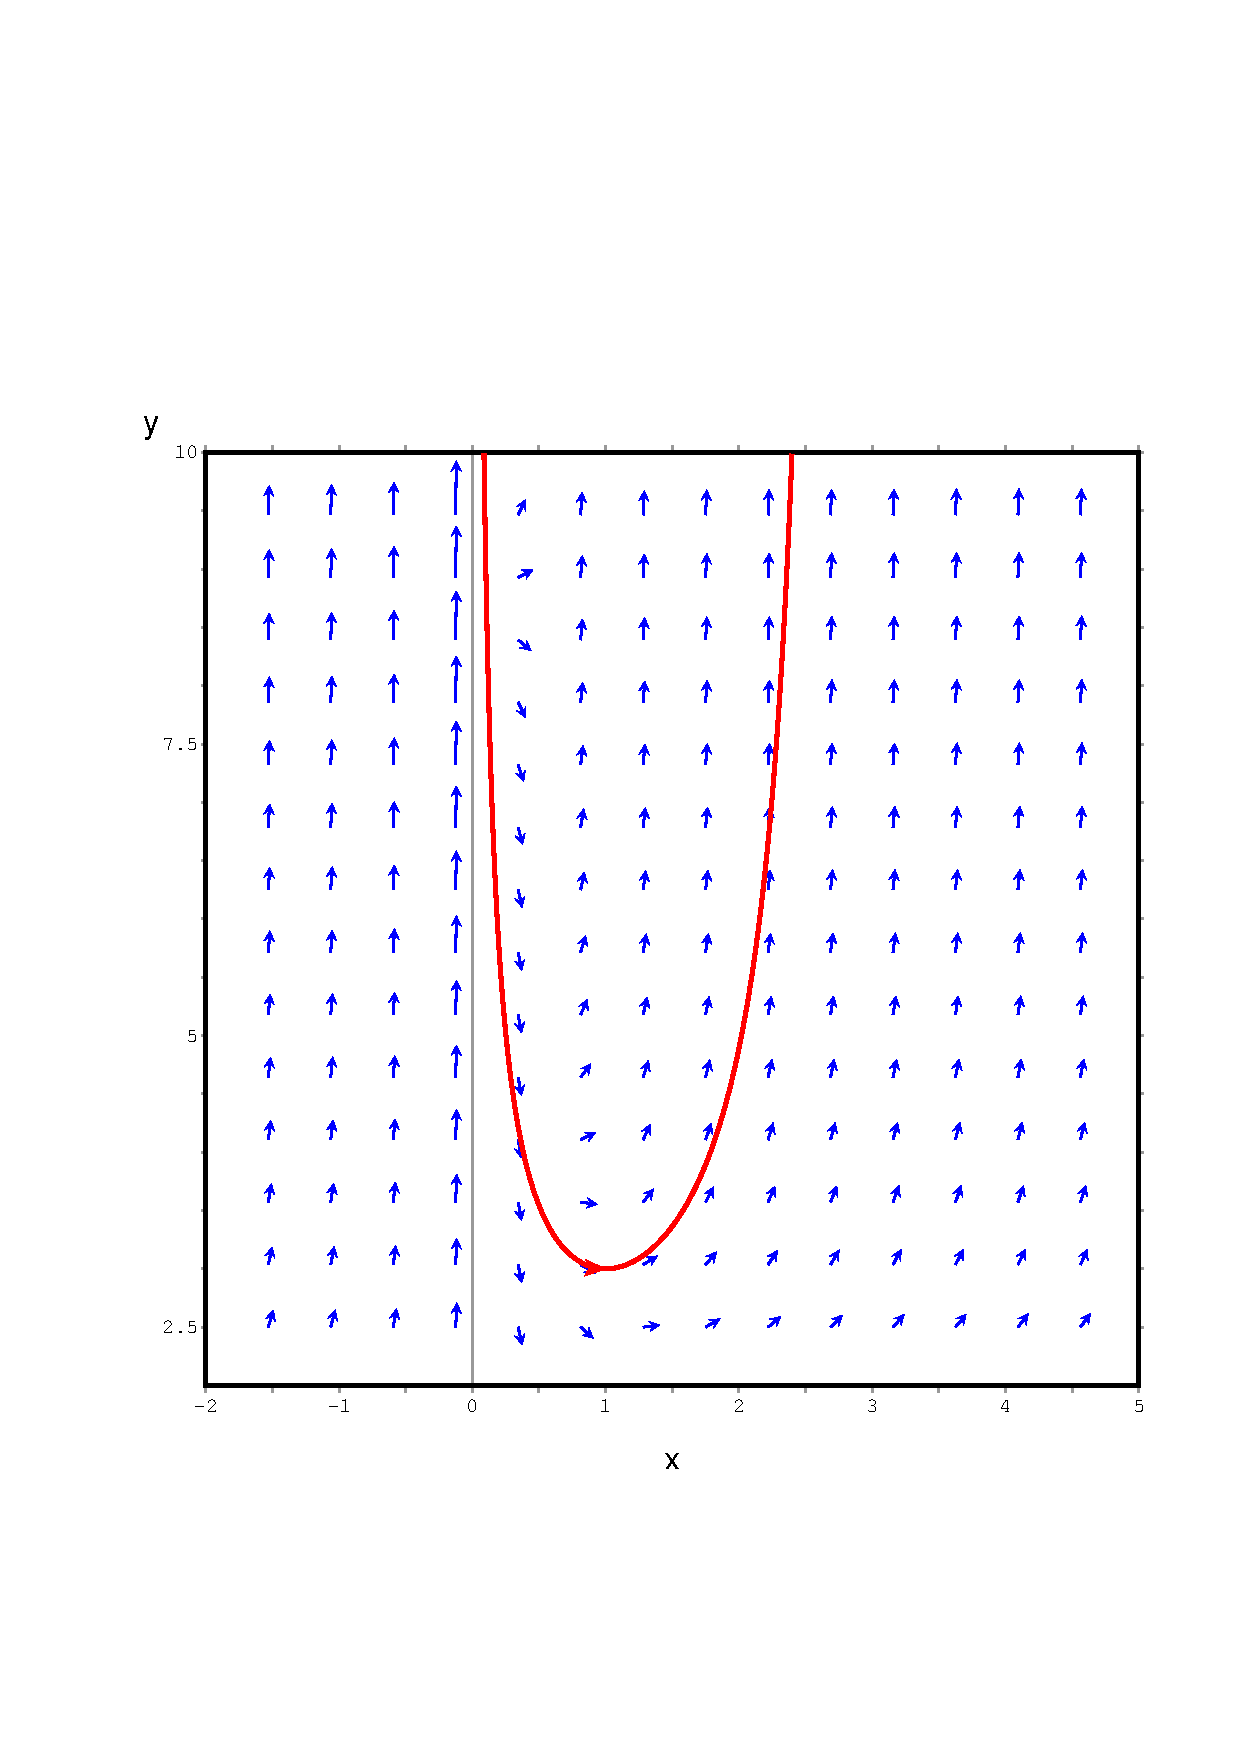
\includegraphics[width=.5\linewidth]{./src/6_}
		\captionof{figure}{Векторное поле уравнения $3(xy' + y) = xy^2$}
		\end{figure}

		\pagebreak
		\item[7.]
		$$(y^{2} + y\sec^{2}{x})dx + (2xy + \tg{x})dy = 0$$
		$$\frac{\partial(y^{2} + y\sec^{2}{x})}{\partial y}  = 2y + \frac{1}{\cos^{2}{x}} = \frac{\partial (2xy + \tg{x})}{\partial x}$$
		\textbf{Тип: }
		$$(y^{2} + y\sec^{2}{x})dx + (2xy + \tg{x})dy = 0$$  Следовательно,  уравнение в полных дифференциалах \\ 
		
		\textbf{Решение: }
		Найти общее решение, которое выражается в элементарных функциях, не удалось \\
		
		\textbf{Команды вводимые в wxMaxima: } 
		\begin{verbatim}
		(y*y+y/(cos(x)*cos(x)))=-(2*x*y+tan(x))*'diff(y, x);
		load('contrib_ode);
		contrib_ode(%, y, x);
		method;
		plotdf(-(y*y+y/(cos(x)*cos(x)))/(2*x*y+tan(x)));
		\end{verbatim}
		\begin{figure}[ht]
		\center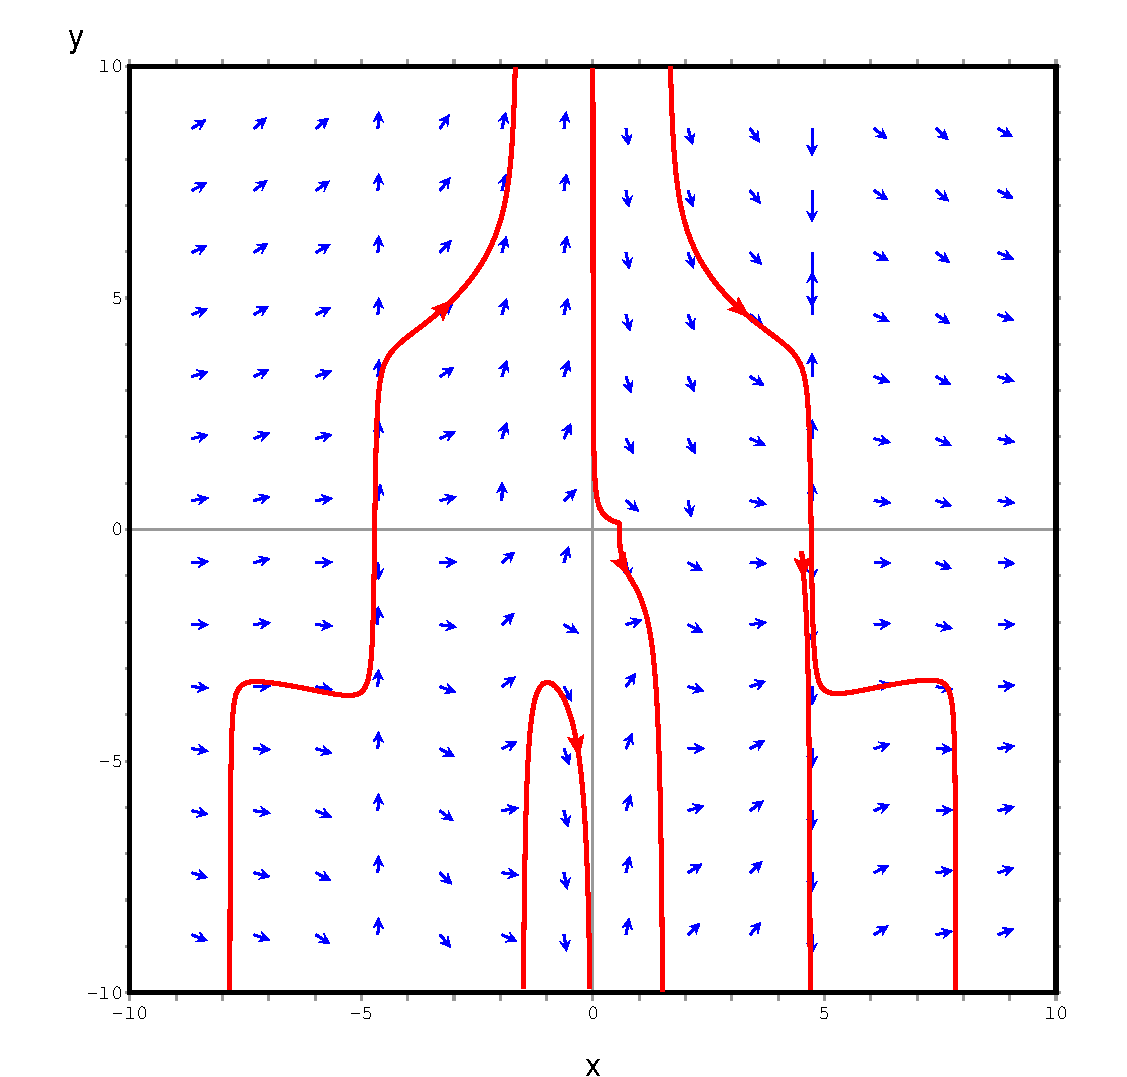
\includegraphics[width=.5\linewidth]{./src/7_}
		\captionof{figure}{Векторное поле уравнения $(y^{2} + y\sec^{2}{x})dx + (2xy + \tg{x})dy = 0$}
		\end{figure}

		\pagebreak
		\item[8.]
		$$y' = \frac{2x}{3y}; \quad M(1, 1)$$
		$$3ydy = 2xdx$$ 
		\textbf{Тип: }
		дифференциальное уравнение 1-го порядка с разделяющимися переменными \\

		\textbf{Общее решение}
		$$\frac{3y^2}{4} = \frac{x^2}{2} + C$$

		\textbf{Частное решение:}
		$$\frac{3y^2}{4} = \frac{1+2x^2}{4}$$

		\textbf{Команды вводимые в wxMaxima }
		\begin{verbatim}
		ode2('diff(y,x)=(2*x)/(3*y) , y, x);
		method;
		ic1(%, x=1, y=1);
		plotdf((2*x)/(3*y), [trajectory_at, 1, 1]);
		\end{verbatim}
		\begin{figure}[ht]
		\center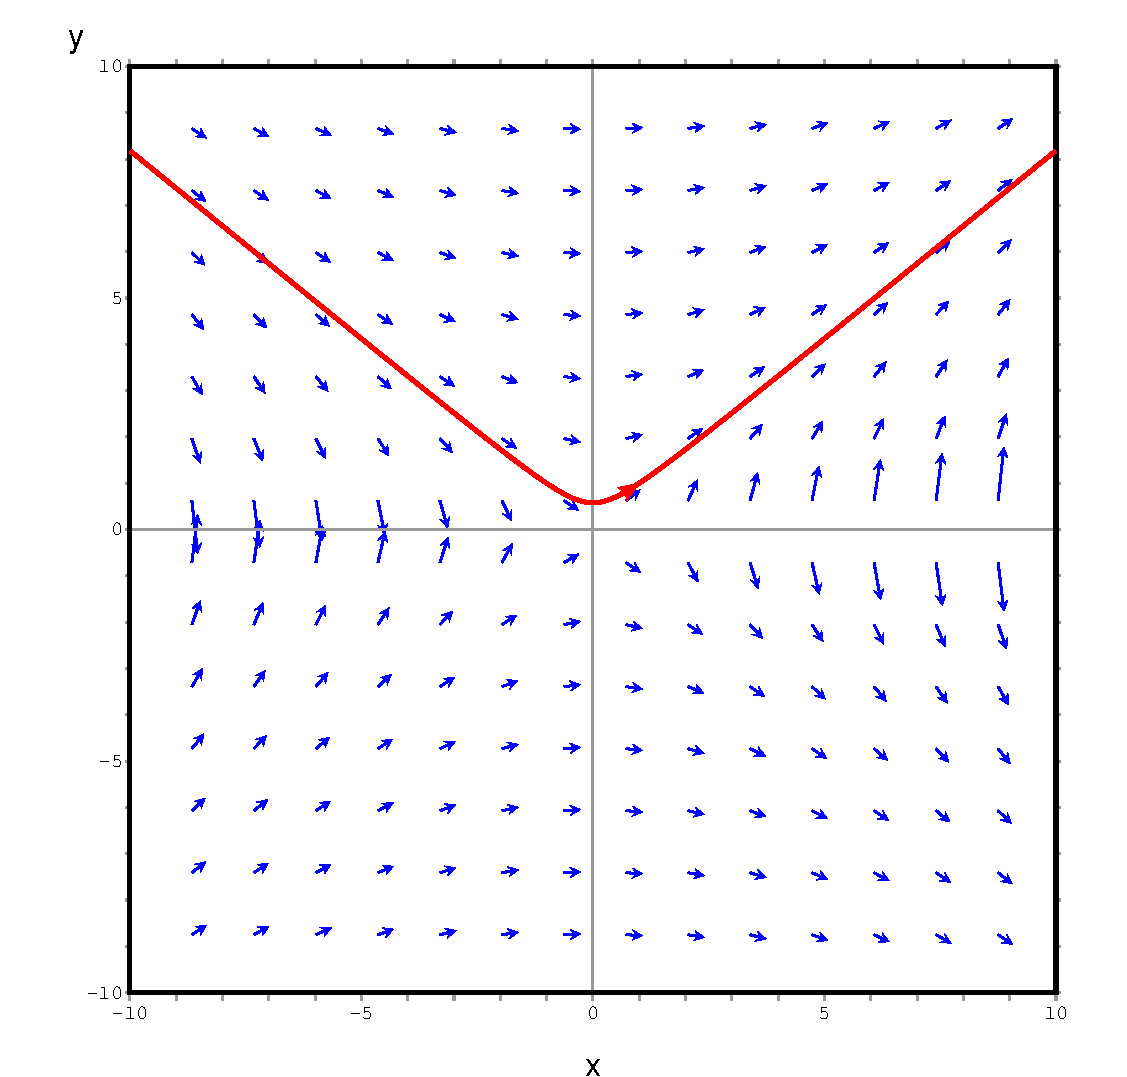
\includegraphics[width=.5\linewidth]{./src/8_}
		\captionof{figure}{Векторное поле уравнения $y' = \frac{2x}{3y}$}
		\end{figure}

	\end{enumerate}

\end{document}